\chapter*{Conclusions}
\chaptermark{}

Figure~\ref{fig:phisDGsNew} shows the current status of $\phis$ and $\DGs$ measurements. It is an update of Figure~\ref{fig:phisDGs} in
Section~\ref{subsec:intro_Jpsiphi_decay}, which gives an overview of the status in the Spring of 2014, when only results with the 2011
dataset from LHCb were available. Results of the measurement presented in this thesis, which uses both the 2011 and 2012 LHCb datasets and
was published in \cite{LHCb-PAPER-2014-059}, are shown in combination with the results from measurements in the
\BstoJpsipipi~\cite{LHCb-PAPER-2014-019} and \BstoDspDsm~\cite{LHCb-PAPER-2014-051} decay channels. The other results in the figure are
from a new CMS measurement~\cite{CMS:2014jxa}, the updated \atlas{} measurement~\cite{Aad:2014cqa}, and the CDF~\cite{Aaltonen:2012ie} and
D0~\cite{Abazov:2011ry} measurements in the \BstoJpsiphi{} channel.
\begin{figure}[htb]
  \centering
  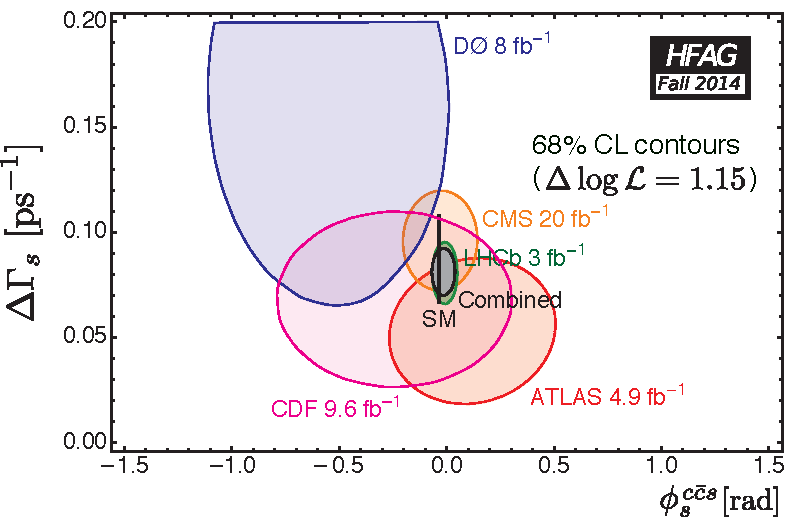
\includegraphics[width=\textwidth]{graphics/results/hfag_Fall2014_DGsphis-cmyk}
  \caption{Combination of $\phis$ (here represented as $\phisccs$) and $\DGs$ measurements by HFAG~\cite{Amhis:2012bh}.
           The estimates at 68\% confidence level (CL) by the different experiments are shown by the coloured contours.
           Note that the LHCb contour (green) is a combination of measurements in the
           \BstoJpsiphi{}, \BstoJpsipipi{}, and \BstoDspDsm{} decays.
           The combined 68\% confidence region is shown by the grey area and the Standard Model prediction by the vertical bar.}
  \label{fig:phisDGsNew}
\end{figure}
